\chapter{Theoretical Background} %%%%%%%%%%%%%%%%%%%%%%%%%%%%%%%%%%%%%%%%%%%%%%%%%%%%%%%%
\label{chap:theoretical_background}

\section{Artificial Neural Networks}

A neural network is inspired from the working of "neurons". Neuron, a biological term, is the fundamental unit of the nervous system and is responsible for transmission of sensory input, sending motor commands to muscles and relaying electrical signals between the different parts of the body. These electrical signals are called action potential and signal the "activation" of a neuron if the potential is above threshold value. The action potential and consequent transmitter release allow the neurons to communicate with other neurons.
\begin{figure}[ht]
\centering
\begin{minipage}{.5\textwidth}
  \centering
  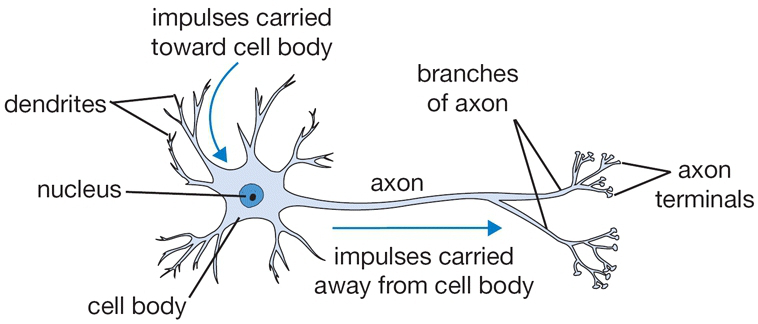
\includegraphics[width=1.2\linewidth, height=3.90cm]{BachelorMasterThesis/TheoreticalBackground/Figures/Biological_Neuron.png}
  \captionof{figure}{Biological Neuron \newline\cite{karparthy}}
  \label{fig:biological_neuron}
\end{minipage}%
\begin{minipage}{.5\textwidth}
  \centering
  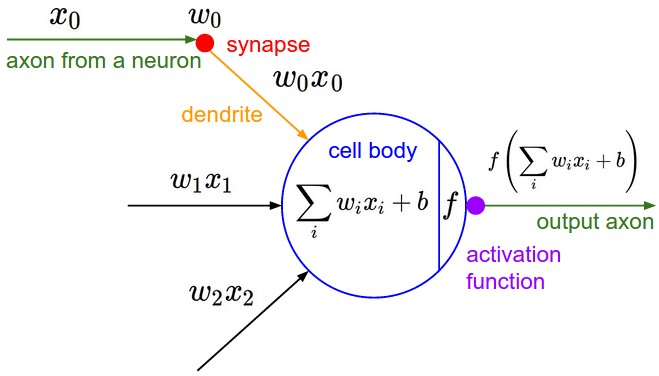
\includegraphics[width=1.0\linewidth, height=4cm]{BachelorMasterThesis/TheoreticalBackground/Figures/Mathematical_Neuron_Model.jpeg}
  \captionof{figure}{Mathematical model of the neuron \cite{karparthy}}
  \label{fig:mathemetical_model}
\end{minipage}
\end{figure}

In the context of Artificial Neural Networks(ANN), a neuron is nothing but a set of inputs, a set of weights, and an activation function. The connections between the neurons are modelled as weights and the activation function is responsible for the magnitude of the output (as shown in Figure~\ref{fig:biological_neuron} and Figure~\ref{fig:mathemetical_model}). 

An artificial neural network consists of at-least 3 layers (shown in~\ref{fig:neural_network}) - the input layer, the hidden layers and the output layer. The initial data to the network is provided through the input layer, the computations are performed and representations are learned in the hidden layers and the output layer produces the result for the given inputs. In general, the formula for computation of activation for a $n^{th}$ layer in a multi-layered neural network is done through:

\[a^n = \sigma(W^n\:.\:\sigma(W^{n-1}\:.\:\sigma(\:.....\:\sigma(W^1\:.\:a^0)\:....\:)))\]

where $\sigma$ is the activation function, $W$ is the combined weight in a layer and $a$ is the activation value at a layer.
\begin{figure}[t]
    \centering
    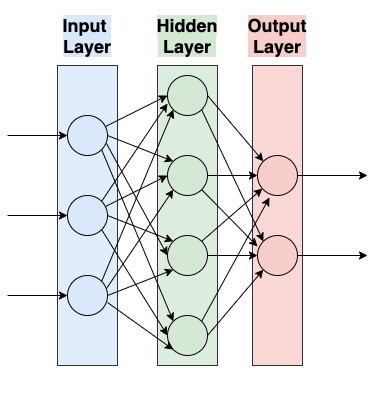
\includegraphics[width=0.7\linewidth]{BachelorMasterThesis/TheoreticalBackground/Figures/A_Simple_NN.png}
    \caption{A simple neural network}
    \label{fig:neural_network}
\end{figure}

Various linear functions as well as non-linear functions such as Sigmoid, tanh (hyperbolic tangent function), ReLU (Rectified Linear Unit), and Leaky ReLU can be used for activation. The most important features for the activation function are:

\begin{itemize}
    \item Non-linearity of the activation function
    \item The function should be differentiable
\end{itemize}

It easy for the model to generalize or adapt with a variety of data and to differentiate between the output by using non-linear activation functions. "Sigmoid" functions (Fig~\ref{fig:sigmoid_fn}) are used in models where we have to predict the probability as an output. This function has a "S"-shaped curve or sigmoid curve. The formula for the sigmoid function is:
\begin{equation}
f(x) = \frac{1}{1 + e ^ {-x}}
\end{equation}

The output from this activation function can then be rounded off to produce binary output (0 or 1). "tanh" is also a logistic function like the sigmoid but the range of the function is (-1 to 1). 

\begin{figure}[ht]
\centering
  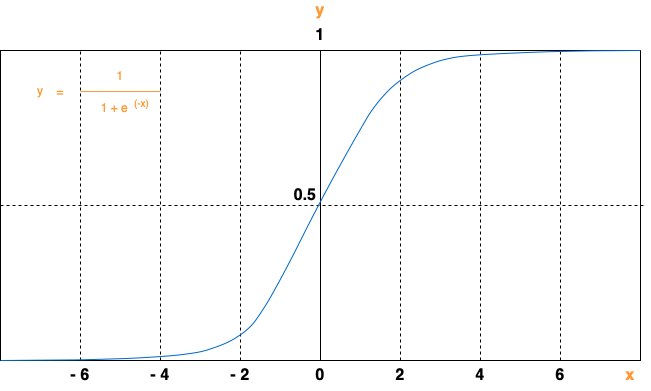
\includegraphics[width=0.7\linewidth, height=5cm]{BachelorMasterThesis/TheoreticalBackground/Figures/sigmoid_fn.png}
  \captionof{figure}{Sigmoid activation function}
  \label{fig:sigmoid_fn}
\end{figure}

ReLU (Fig~\ref{fig:ReLU_fn}) is one of the most used activation function whose range is [0 to infinity). Using this function, the negative values become zero. This is computationally very cheap and and sparsely activated. This activation function also has a better gradient propagation with less vanishing gradient problem. The formula for the ReLU function is: 

\begin{equation}
 y = max(0, x)
 \end{equation}

\begin{figure}[ht]
  \centering
  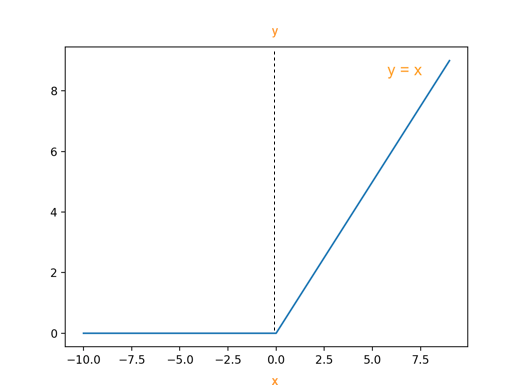
\includegraphics[width=0.8\linewidth, height=5cm]{BachelorMasterThesis/TheoreticalBackground/Figures/Relu_Activation.png}
  \captionof{figure}{ReLU activation function}
  \label{fig:ReLU_fn}
\end{figure}

\clearpage
\section{Convolutional Neural Network (CNN)}

One of the first self-learning neural network model was developed by Fukushima, called "Neocognitron"\cite{fukushima1980neocognitron}. The Neocognitron had an extended hierarchy structure and was inspired by the visual nervous system model proposed by Hubel and Wisel in the early '60s. Fukushima talks about a neural network model in his paper that performs self-learning for visual pattern recognition by unsupervised learning. Fukushima mentions the use of modular structures and cells which are connected by cascading and preceded by an input layer. He also mentions two types of layers -  convolutional layers and downsampling layers. According to this paper, such types of networks could recognize a pattern with position-invariance.

If there is high position-invariance, as is the case in daily life pattern recognition problems, it becomes important to identify an appropriate set of features. If such features are identified, then the position of features become less important. As mentioned in the paper by LeCun et al. \cite{lecun1999object} Convolutional Neural Networks(CNNs) can be designed to perform such tasks. CNNs can be used to recognise patterns without explicitly segmenting the data. CNNs can thus be considered to be good feature extractors. This is typically the case in the field of computer vision \cite{athiwaratkun2015feature}, for time series data \cite{yang2015deep} and are also often deployed for the medical data \cite{pyakillya2017deep}.

The convolution layer (ConV) is the nucleus of CNNs. The convolutional layer's parameters consist of a set of learnable filters, sometimes also called kernels. These filters have a small receptive field \cite{karparthy}. During the forward pass, we convolve across the spatial position of the input volume and we compute the dot product between the entries of the filter and input at any given position. As we slide over the input, the filter produces a feature map that gives the responses of that filter at every spatial position. The network will thus become aware of those filters, which activates when features are detected. 

In principle, we have multiple feature maps that learn different features. These feature maps are stacked together to produce the output volume. Thus, every entry in the output volume can be interpreted as an output of a neuron that looks at a small region in the input. %and shares parameters with neurons in the same feature map.

\begin{figure}[ht]
    \centering
    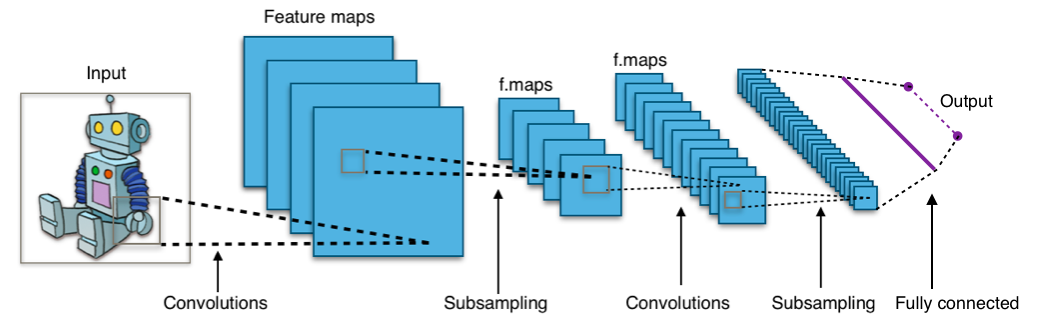
\includegraphics[width=1.0\linewidth, height=6cm]{BachelorMasterThesis/TheoreticalBackground/Figures/Typical_CNN_Architecture.png}
    \caption{CNN Architecture \cite{wiki:xxx}}
    \label{fig:a_cnn_architecture}
\end{figure}

The other important layers of the CNN network are the pooling layers. A pooling layer is a non-linear method of downsampling. Pooling layers are important because downsampling does not change the input, thus incorporating translation invariance. It decreases the spatial dimensions, thus reducing the number of parameters and the amount of computation in the network. Also, pooling computation is independent of the depth of the input. Most common pooling functions are max-pooling, average-pooling, $l_2-norm$ pooling, region of interest(ROI), etc. A regular CNN architecture incorporating these layers is shown in Figure ~\ref{fig:a_cnn_architecture}

Mathematically, if the data is single dimensional and if the ConV layer accepts an input of size $W \times D$ ($timesteps \times features$), then the ConV layer produces an output of volume $W_1 \times D_1$, where $W_1$ and $D_1$ are calculated as follows:

\[ W_1 = ( (W - F + 2P) / S) + 1 \]
\[ D_1 = K \]

where $K$ is the number of filters, $F$ is the filter size or spatial extent, $P$ is the padding and $S$ is the stride used during convolution. The number of filters is typically a power of 2, whereas the padding is used to control the spatial dimension of the output volume. Stride controls how the filter convolves over the input volume.

The number of parameters for a layer is the count of “learnable” elements. These are learnt during training and the number is calculated as follows:

\[\text{Number of parameters} = F \times D \times D_1\]

These parameters are added for all the layers of the model in the end and are called trainable parameters. 

\clearpage
\section{Deep Neural Network (DNNs) for specialized hardware}

Convolutional neural networks are a subclass of deep neural networks. Most modern deep learning networks use multiple layers progressively to extract higher-level features from the input. But these multi-layered neural networks are commonly large, complex and involve usage of a considerable amount of resources to train and evaluate the dataset. Such complex and intensive networks can result in very long processing times on standard x86 CPUs. Specialized hardware such as graphical processing units (GPUs), application specific integrated circuit (ASIC) and field programmable gate arrays (FPGAs) become essential for such tasks. Specialized hardware can improve the processing capabilities and performance of deep learning models. Computing tasks on specialized hardware would decrease the latency and increase throughput. As such, specialized hardware can be used to train the deep learning models. We speak about FPGAs and GPUs in the next section.

\subsection{FPGAs vs GPUs}

A GPU is a specialized hardware with a highly parallelized structure which makes them more efficient than general-purpose CPUs for heavy computing problems. GPUs have orders of magnitude more computational cores when compared to CPUs. Researchers from Stanford explored the usage of GPUs for training CNNs \cite{coates2013deep} and found that GPUs can be leveraged to perform more arithmetic operations per second to train large CNN networks. This would decrease the time for training and inference.

The other class of specialized hardware is the FPGAs. FPGAs contain an array of re-programmable logic blocks that can be configured to perform complex combinational operations with arbitrary precision. FPGAs are re-configurable integrated circuits and can be reprogrammed to implement different logic functions. This is different from instruction based hardware such as GPUs and CPUs, which are configured through software. An early publication of the usage of FPGAs was by Microsoft researchers. They used FPGAs to accelerate the search of "Bing" (which is using CNNs) by a factor of nearly 2X in their datacenters \cite{ovtcharov2015accelerating}.

FPGAs have further advantages when compared to GPUs and CPUs. GPUs are typically connected as a co-processor to CPUs. For any practical use case, it requires assistance from the CPU, whereas FPGAs can be directly connected to any data source, such as a network interface, sensors, or other interfaces. FPGAs can be configured to directly access hardware I/O without the latency of internal bus structures which gives high bandwidth and low latency for the FPGAs. But, GPUs can execute thousand of arithmetic operations parallelly and brute-force throughput of GPUs should not be underestimated. 

Many recent studies in the field of computer vision have shown that FPGAs are known to outperform GPUs in terms of energy consumed per frame as the complexity of the pipelines grow \cite{qasaimeh2019comparing}. But considering the constrained on-chip resources on FPGAs, the DNN model must be optimized for energy efficiency. DNNs can be optimized with number of operations that would translate into energy required for a single classification action. But, it is not very easy to design the DNN models which would take into account these constraints of FPGAs. DNNs can be fairly large in size which can become an issue on FPGAs. This leads to a discussion of the next topic - AutoML.

\section{AutoML}

Traditionally, machine learning model development is resource-intensive and requires significant domain knowledge and effort. Then comes the process of experimenting with various models, preprocessing and data augmentation. The layers of the DNN would have to be modified to see if the model performance improves and then to find suitable hyperparameters for the model. Thus, the success of DNNs depends on the proper configuration of its architecture and hyper-parameters. As such the entire process is tedious. Such problems led to the development of the concept of AutoML. AutoML has the goal to automatically search for an optimal DNN and automating the tasks across the end-to-end ML pipeline.

The process to automate DNN's configuration is rather a compelling thought. By this approach, we can find innovative DNN configurations that might not be possible by standard design techniques. We can also find configurations that are practical to be implemented on specialized hardware such as the FPGAs, and this becomes possible without the domain expertise.

\subsection{Neural Architecture Search (NAS)}

As discussed, finding a DNN model requires significant architectural engineering. It might not be convenient to design such a network, considering that it requires a fair amount of trial and error and experimentation which is time-consuming. This is where Neural Architecture Search (NAS) comes in. NAS is a subset of AutoML which can be used to find various DNN architectures.

\begin{figure}[ht]
    \centering
    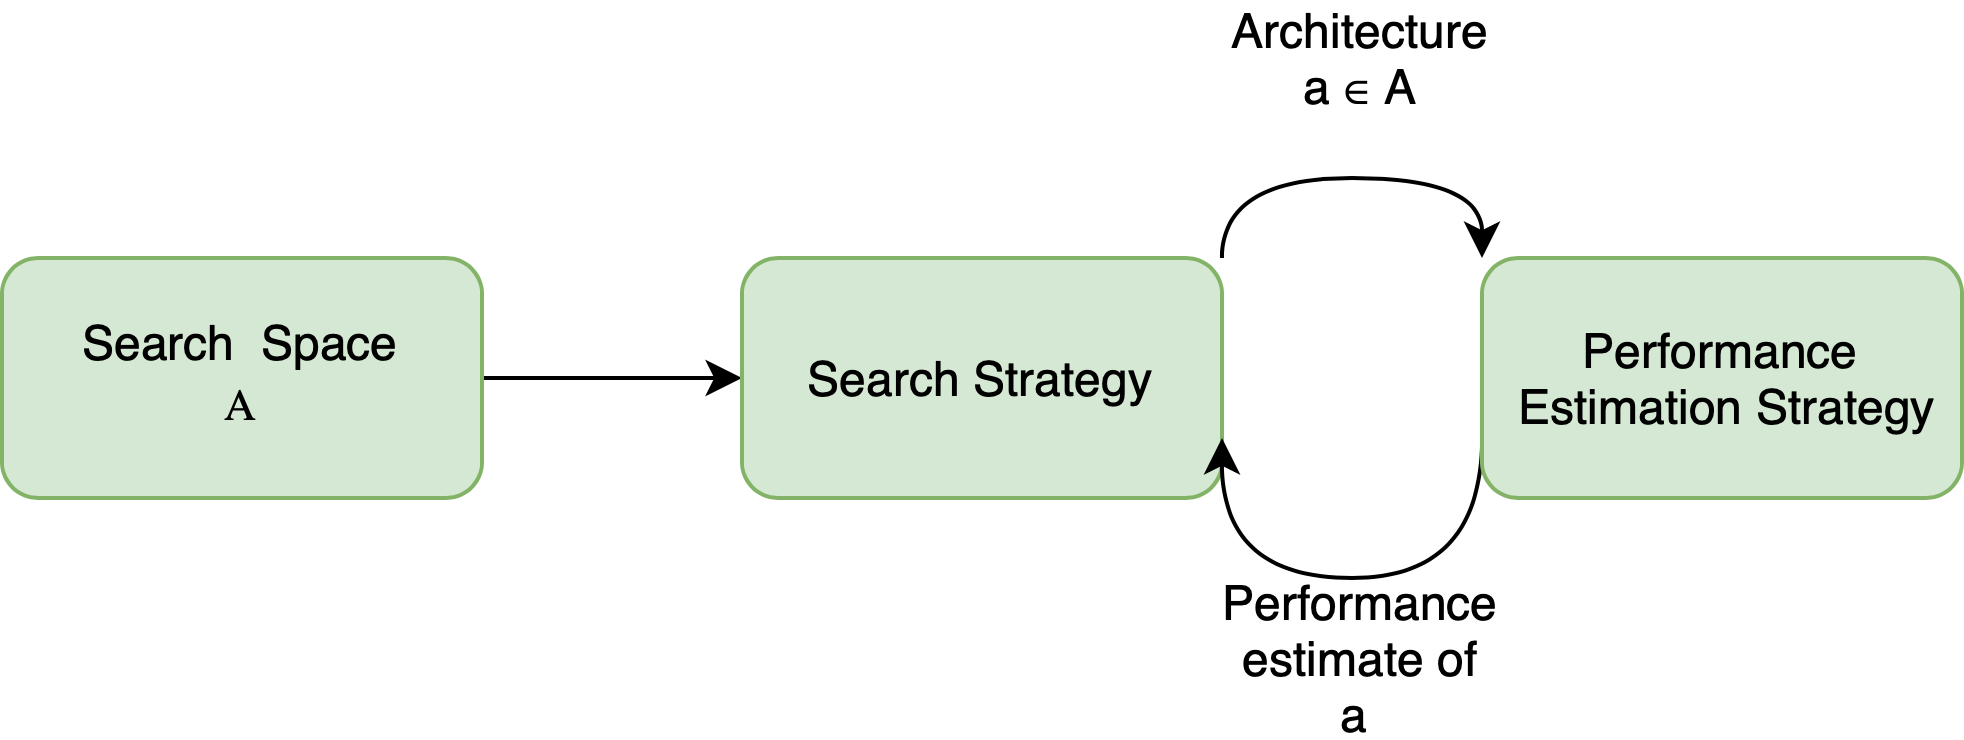
\includegraphics[width=1.0\linewidth, height=4cm]{BachelorMasterThesis/TheoreticalBackground/Figures/NAS_strategy.png}
    \caption{NAS method illustration \cite{elsken2018neural}}
    \label{fig:nas_method_illustration}
\end{figure}

There are essentially 3 steps which is used in NAS (as shown in ~\ref{fig:nas_method_illustration}):
\begin{itemize}
    \item Search Space: This is the set of all feasible solutions for the given problem. It defines the set of architectures that can be represented in principle. In general, the search space is huge. It is essential that the size of the search space is reduced by incorporating prior knowledge of architectures well suited for a task even if this introduces human bias.
    
    \item Search Strategy: This step defines the approach on how to explore the search space. There are many search strategies that can be used such as the random search, the Bayesian optimization, reinforcement learning, and the evolutionary methods. While deciding the search strategy, exploration-exploitation trade-off to find well-performing architectures or to find models quickly needs to be considered. 
    
    \item Performance estimation strategy: This defines the guiding criteria for the NAS to select a DNN as the best performing DNN. The simplest way of achieving this is to train the DNN for the training data and evaluate the performance on the validation data. Accuracy, for example, can be used as the guiding criteria in image recognition tasks. 
\end{itemize}

\subsection{Genetic Algorithm}
\label{sec:genetic_algorithm_background}

Genetic programming or genetic algorithms are inspired by the biological evolutionary system and can be used for evolving DNNs in machine learning. Genetic Algorithms were developed by John Holland, his students and colleagues at the University of Michigan, most notably David E. Goldberg. Based on such foundations of neural evolution of DNN topologies, today, many groups such as Google's DeepMind, Uber Labs, etc. work on the genetic algorithms on a large scale.

A typical genetic cycle is shown in figure~\ref{fig:genetic_evolution_cycle}. Initially, while starting with the genetic algorithms, either a seed DNN can be used as a parent or a random set of DNNs can be generated. This is followed by a selection of the fittest DNN/DNNs for reproduction (crossover) and mutation according to a predefined fitness measure. Mutation involves the creation of new DNNs, which are also evaluated. 

\begin{figure}[t]
    \centering
    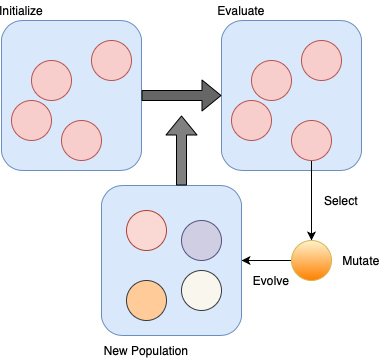
\includegraphics[width=0.7\linewidth, height=8cm]{BachelorMasterThesis/TheoreticalBackground/Figures/Evolution_Cycle.png}
    \caption{A typical Genetic Evolution cycle}
    \label{fig:genetic_evolution_cycle}
\end{figure}

\begin{itemize}
    \item \textbf{Initialize}: A seed DNN model or an initial set of DNN topologies is created at random. This is the initial set of a population of possible solutions that needs to be evaluated.
    \item \textbf{Evaluate}: This is the stage when the DNN topologies are evaluated. The evaluation is done on the performance estimation strategy. Different performance measures can be used. The most common one used for image recognition tasks is the accuracy of the DNN topology. 
    \item \textbf{Selection}: This is the stage in which DNN topologies are selected from a population for later breeding (mutation). The selection may take place through the evaluation of a fitness function for individual DNN topology. This kind of selection is called fitness-based selection. One (single parent) or more than one (multiple parents) DNNs can be selected for the process of mutation. Such a selection mechanism is very robust as better-performing DNNs have a chance of being selected for mutation. But such a selection process has the problem that it might lead to slower convergence for the selection of final DNN topology. 
    \item \textbf{Mutate}: The process of producing the new topologies is called mutation. Mutation, in general, involves substituting some part of a DNN topology with another part. Mutation maintains the genetic diversity from one generation to another. After selecting the DNN for the mutation process, new DNN topologies are produced from the selected topology. The new DNN topologies belongs to the new population and is called a new generation. There are many methods to mutate and produce a new generation. This is a recursive process until a specified number of generations is produced.

    The goal of the genetic algorithms is to improve the performance of the DNN over generations. The selection process should select one or more new parent topologies. Mutation also follows certain policies such as random mutation, smart and selective mutation, etc. After mutation, the performance of a DNN may change entirely from the previous DNN. Depending on the kind of mutation, members of the new generation are generally more fit than the previous generation, although this is not always true. 
    
    A simple example of mutation can be demonstrated as below. If we consider a set of bits as the genes of a parent, then flipping just one of the bit will result in a new child. The flipping of the bit can be at any random position and the resulting child might produce a completely different solution. If we were to find an analogy between the set of bits with that of a DNN, then the bits can be compared to layers of the DNN.
    
    \clearpage
    
    \textbf{Parent}: 
    
    1 0 0 1 0 0 \textbf{\textsl{0}} 1
    
    \qquad\quad\qquad$\Big\downarrow$ mutation
    
    1 0 0 1 0 0 \textbf{\textsl{1}} 1
    
    \textbf{Child}
    
\end{itemize}
    
    Genetic algorithms have various advantages. These algorithms have very good parallel computing capabilities. The siblings in the new generation can be trained in parallel as there is no dependency between those. Genetic algorithms are also known to optimize both continuous and discrete functions and can provide a list of good solutions instead of only one. Genetic algorithms are also known to always produce a solution.
    
    From a mathematical perspective also, genetic algorithms perform very well. Typical machine learning methods provide solutions to a problem that are locally optimal. This means there can be an improvement to the solution but there is a tendency to not scrutinize it. Since genetic algorithms are iterative, they tend to explore more than one solution and can provide a global solution (as shown in~\ref{fig:objective_function}).
    
    Genetic algorithms can be pretty noisy as they generate many bad networks. But this can be used as an advantage for exploration. This can be achieved by controlling the extent of the mutation. For a network which produces good results, the extent of mutation should be low, where as if a network produces bad results, then mutation should be high.
    
\begin{figure}[ht]
    \centering
    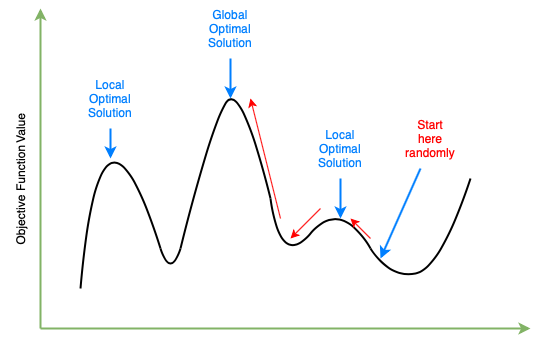
\includegraphics[width=1.0\linewidth, height=6cm]{BachelorMasterThesis/TheoreticalBackground/Figures/Objective_Function.png}
    \caption{Genetic Algorithm methodology}
    \label{fig:objective_function}
\end{figure}

\subsection{Optimization Criteria}

The performance of a neural network depends on several factors. Generally, the network architecture takes the spotlight for the performance, but optimization algorithms also play an important part. Mathematically speaking, optimization algorithms are used to minimize an objective function. The objective functions are dependent on the internal learnable parameters of the model such as the weights and the bias. These learnable parameters are used to compute the target values for the problem. The learnable parameters compute the output values and these parameters are updated in the direction of optimal solution i.e. minimizing the loss during the training process.

Today, the most general way to train a deep neural network model is by using gradient descent optimizer or by using one of its variants such as Adam, RMS, AdaGrad, etc. The generic formula for gradient descent is:
\newline
\[\theta=\theta - \eta . \nabla J(\theta)\]
\newline
where $\eta$ is the learning rate and $\nabla J(\theta)$ is the gradient of loss function $J(\theta)$, $\theta$ being the parameters.

In simple words, we use a metric and a method that maximizes or minimizes this metric for the given data. This metric could be accuracy or precision/recall (used for image and text data), or detection rate and false alarm rate (used for ECG data for arrhythmia detection). Our model, with learnable parameters, will try to search and optimize these parameters to maximize or minimize the metric for the data.

Since NAS is an iterative process, it is associated with one or more stopping criteria. This iterative process is stopped when the stopping criteria is met. In every generation of NAS, we can look for one or more topology with the best metric values and continue this iterative process of producing a new generation until the stopping criteria is met. The stopping criteria can based not only on metrics such as accuracy, precision/recall, etc but also on the parameters such as number of generations of evolution or remaining active number of topologies. 

When building DNNs for hardware such as the FPGAs, it is also important to consider the resource consumption as an optimization criteria. Resource consumption can be interpreted as the number of floating-point operations (FLOPs) and the data access which would translate into energy consumed, as previously explained. This way, the number of parameters and number of FLOPs can also be considered as an optimization criteria.
% \newpage 

% \subsection{Hyper-parameter optimization}   \todo[inline, color=yellow]{I think i should remove this section as we have not done this. Should i?}

% Hyper-parameters, by definition are those parameter values that can be additionally used to control the machine learning process to train a Neural Network model. These parameter values are sometimes also called measures or constraints. By contrast, the model parameters are those values that are learned during the learning process. To generalize different data patterns, the same model can require different constraints and learning rates. These constraints have to be tuned to minimize the predefined loss function on the given data to find an optimal model.

% There are various approaches for hyper-parameter optimization and can separate into an exhaustive search of the space and surrogate model techniques. The traditional approach has been grid search or parameter sweep. This is a simple exhaustive searching technique through a manually specified subset of the hyperparameter space. This kind of algorithm must be guided by performance metrics.

% The other approach is gradient-based optimization. The logic to compute the gradient with respect to hyperparameters and then optimize the hyperparameter using gradient descent. This approach was first used for neural networks and then extended for other techniques such as support vector machines(SVMs). 

% Bayesian optimization, a surrogate technique, is also another method used for hyperparameter optimization. It is considered to be a global optimization method as it can be used for noisy black-box functions. Bayesian optimization builds a probabilistic model. By evaluating a hyperparameter configuration iteratively, this method aims to accumulate observations revealing as much as information as possible about this black-box function, especially the location of the minimum. It tries to balance exploitation and exploration.

% Another approach for hyperparameter optimization is using evolutionary algorithms. This is also a global optimization technique for black-box functions in which the evolutionary algorithms search the space of hyperparameters. This process is also inspired by the biological concept of evolution and used for statistical machine learning, neural architecture search as well as training of the weights for deep neural networks. 

% One of the newer methods for hyperparameter optimization is Population Based Training(PBT) presented in \cite{jaderberg2017population}. PBT tries to merge exhaustive and parallel methods. This method can adapt and tune hyperparameters in a decentralised and asynchronous method. PBT starts with randomly sampling hyperparameters and weight initialisations and evaluating the performance periodically and asynchronously. Mathematically speaking, we try to optimize the parameters $\theta$ of a model $f$ to maximize a given objective function, but with the additional constraint to search over multiple possible hyperparameter values $h$ \cite{jaderberg2017population}.

% $$\theta^* = optimize(\theta|h^*), h^* = \argmin_{h \in \mathcal{H^T}} eval(optimise(\theta|h)) $$

% \todo[inline, color=yellow]{Can use PBT for hyperparameter optimization for our NAS. It can be really useful. - We are now}

% \begin{figure}[ht]
%     \centering
%     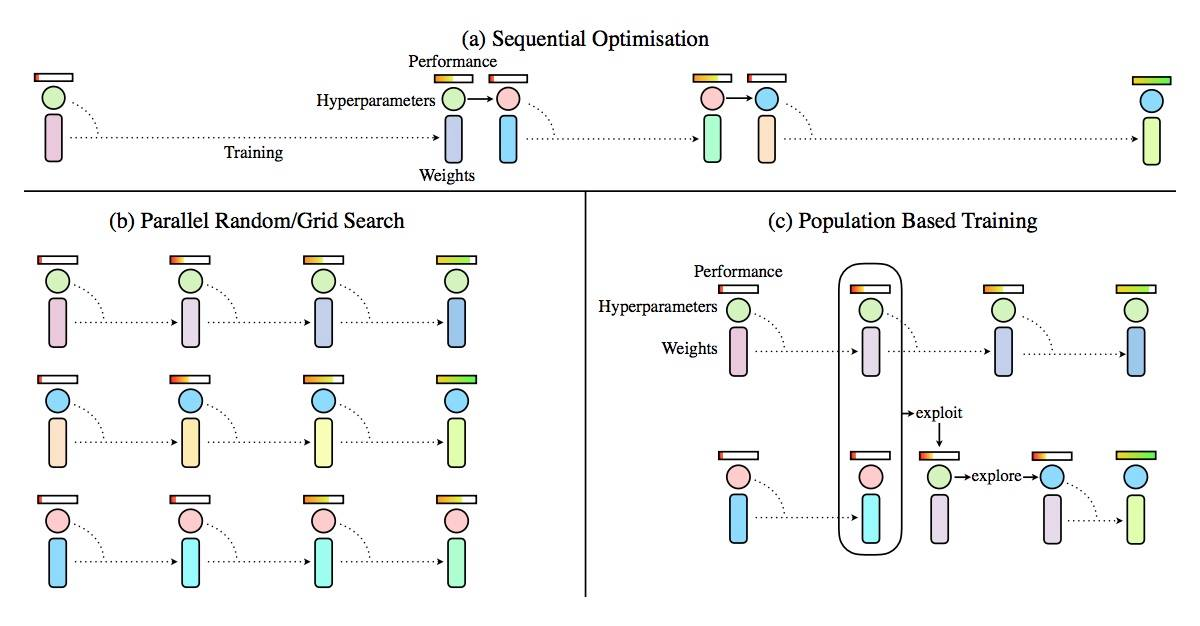
\includegraphics[width=1.0\linewidth, height=7cm]{BachelorMasterThesis/TheoreticalBackground/Figures/Hyperparameter_optimization.jpg}
%     \caption{Common paradigms of tuning hyperparameters: sequential optimisation and parallel search (a) Sequential optimisation requires multiple training runs to be completed (potentially with early stopping), (b) Parallel random/grid search of hyperparameters trains multiple models in parallel with different weight initialisations and hyperparameters, (c) Population based training starts like parallel search, randomly sampling hyperparameters and weight initialisations. \cite{jaderberg2017population}}
%     \label{fig:Hyperparameter_optimization}
% \end{figure}

% \section{Quantization}

% Quantization is a concept that refers to the process of reducing the number of bits that are used to represent a number. This essentially means that quantization can be used to reduce bandwidth and storage. In the context of neural networks and deep learning, the predominant storage format used for weights and biases has been 32-bit floating-point or FP32. And the eagerness for better computation efficiency and decrease for bandwidth consumption has lead to research into using lower precision numerical formats for deep learning models. For instance, using INT8 for weights, activations and biases consumes 4x less overall bandwidth compared to FP32. Additionally, integer computations are faster compared to floating-point computations and the hardware will consume less area and is also energy efficient.

% \begingroup
% \setlength{\tabcolsep}{10pt}
% \renewcommand{\arraystretch}{1.5}
% \begin{table}[ht]
%     \centering
%     \begin{tabular}{|c|c|c|}
%         \hline
%         INT8 Operation & Energy Saving vs FP32 & Area Saving vs FP32 \\
%         \hline
%         Add & 30x & 116x \\ 
%         \hline
%         Multiply & 18.5x & 27x \\
%         \hline
%     \end{tabular}{}
%     \caption{Energy and Area saving of INT8 vs FP32 \cite{dally2015high}}
%     \label{tab:int8_vs_fp32}
% \end{table}
% \endgroup

% Quantization, typically, without re-training the DNN model can result in a relatively low loss of accuracy. This might or might not acceptable depending on the use case. To improve accuracy, certain fine-tuning can be used. One such method is called scale factor, which can be used to adapt the dynamic range of the tensor from FP32 format to an integer format. This scale factor can be calculated per-layer but can be further used per-tensor as well. Mapping the min/max values of the float tensor to the min/max of the integer format is the simplest way. 

% We can use quantization during different phases in an ML pipeline as well. During the training phase, we can apply quantization for weights and biases to use FP32 or if relatively low loss of accuracy is permitted, FP16 as well. Whereas, during the inference phase, INT4 or INT8 might be acceptable if the there are relatively few number of classes for classification.

% Research has been carried in the field of developing quantization techniques for hardware-specific implementations of neural networks as well \cite{choukroun2019low}. FPGAs play out its strength for quantization as they are not limited standard floating-point precision like FP32 format or FP16 format, but can be used to represent any number of bits - such as 6-bit values. A toolbox for quantization for Tensorflow operations, emulating fixed point operations in addition to layer wise quatization is demonstrated in \cite{loroch2017tensorquant}. 

